% !TeX root = ../../../master.tex

\subsection{Signup}
\label{ssec:Signup}

Um an einer Umfrage erstellen zu können, muss zuvor ein Nutzerkonto erstellt werden. 
Hierfür wählt der Benutzer wie in \abb \myRefGeneral{fig:SignupImplement} dargestellt das Formfeld mit seinem Benutzernamen wie \zb \emph{\texttt{Sascha}}, den Registerkey, der vom Administrator der Software eingetragen wurde. Dieser könnte \emph{\texttt{DemoKey}} sein.
Anschließend wählt der Benutzer ein Passwort seiner Wahl.
Darauf hin startet er den Registrierungsprozess durch das Drücken des Buttosn \jinline|Sign Up|.
Ist das gewählte Passwort konkludent, so soll der Benutzer auf die \emph{Result-Seite} weitergeleitet, da diese im späteren Verlauf \ua das Kernstück darstellt (siehe Kap. \vref{ssec:ResultDashboardImplement}). 
Stimmt das Passwort nicht überein, so erhält der Benutzer ein visuelles Feedback mit der Aufforderung, seine Passwortwahl erneut einzugeben. 

\begin{figure}[hp]
	\centering
	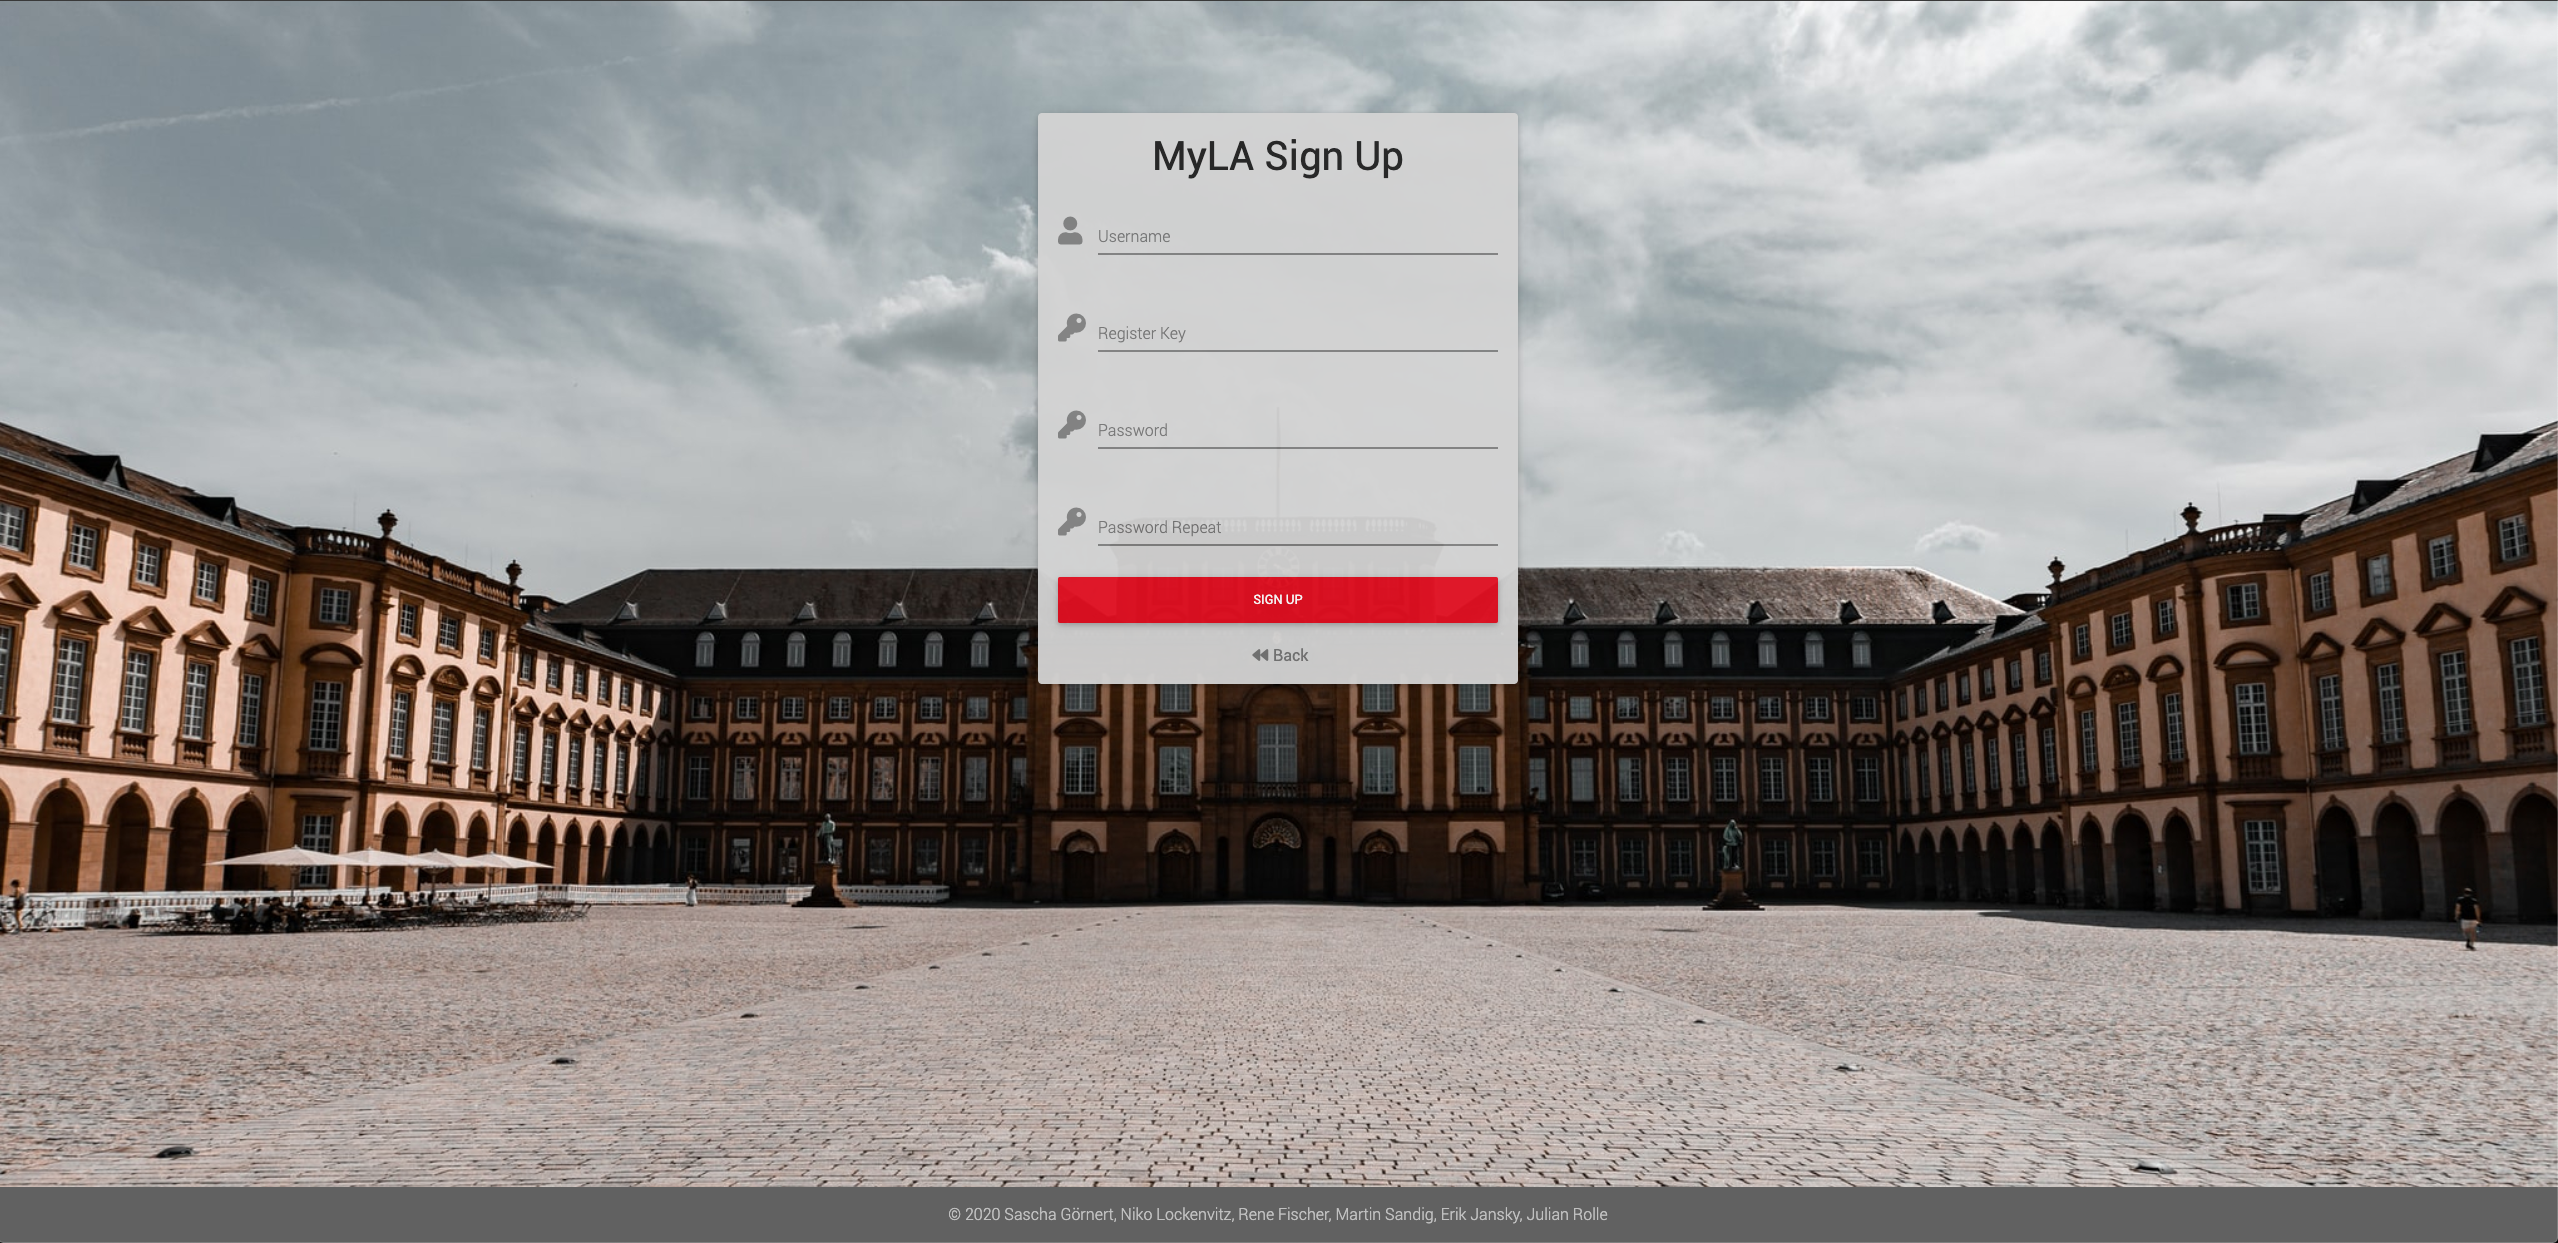
\includegraphics[width=0.95\textwidth, keepaspectratio]{img/client/Signup.png}
	\captionsetup{justification=centering, format=plain}
	\caption[\acf{UI}: Registrierung]{\acf{UI}: Registrierung \\ \quelleScreenshot}
	\label{fig:SignupImplement}
\end{figure}